\documentclass[conference]{IEEEtran}
\IEEEoverridecommandlockouts
\usepackage{iftex}
\ifXeTeX  % Tectonic/XeTeX: Times clone; under pdfLaTeX IEEEtran uses Times itself
  \usepackage{fontspec}\setmainfont{texgyretermes}[Extension=.otf, UprightFont=*-regular, BoldFont=*-bold, ItalicFont=*-italic, BoldItalicFont=*-bolditalic]
\fi
\usepackage{cite}
\usepackage{amsmath,amssymb}
\ifXeTeX\usepackage{unicode-math}\setmathfont{texgyretermes-math.otf}\fi
\usepackage{graphicx}
\usepackage{booktabs}
\usepackage{multirow}
\usepackage{xcolor}
\usepackage{tikz}
\usetikzlibrary{positioning,arrows.meta,fit}
\usepackage[hidelinks]{hyperref}
\usepackage{balance}

\newcommand{\FinalMacro}{0.9134}
\newcommand{\FinalAcc}{98.21}
\newcommand{\ReproMLR}{0.8967}
\newcommand{\PaperMLR}{0.8949}
\newcommand{\CalT}{0.133}
\newcommand{\EceRaw}{0.0041}
\newcommand{\EceT}{0.0070}
\newcommand{\RejCov}{95.2}
\newcommand{\RejAcc}{99.72}
\newcommand{\RejMacro}{0.9861}
\newcommand{\SeedStd}{0.012}
\newcommand{\GainOverRepro}{+0.0168}

\makeatletter\newcommand{\tabinput}[1]{\@@input #1 }\makeatother
\newcommand{\Bfit}{B_{\mathrm{fit}}}
\newcommand{\Bval}{B_{\mathrm{val}}}

\begin{document}

\title{Stacking Handcrafted and Convolutional Features for Wafer Map Pattern Classification, Revisited: Reproduction, Meta-Training Pitfalls, and Improvements}

\author{\IEEEauthorblockN{Kartikeya Gupta}
\IEEEauthorblockA{Indian Institute of Information Technology Sri City\\
Sri City, Andhra Pradesh, India\\
\texttt{kartikeyagupta.r24@iiits.in}}}

\maketitle

\begin{abstract}
Kang and Kang (2021) proposed classifying wafer map defect patterns with a stacking ensemble that combines a
feed-forward network on 59 handcrafted features with a VGG-style convolutional network, merged by a multi-response
linear regression (MLR) meta-classifier. We present an independent reproduction of all six models of that study on the
WM-811K dataset at four training-set sizes, and a set of controlled extensions. At full data, our reproduction reaches a
macro-F1 of \ReproMLR{} for Stacking-MLR against the reported $0.8949 \pm 0.0121$, and matches the remaining baselines.
The reproduction exposed one pitfall: when the meta-classifier is trained on the base classifiers' predictions for their
own training data, as in the public reference code, it learns to trust over-confident outputs and ignores the rarest
class. Training it on a held-out split resolves this, and the same mechanism explains two departures from the original
results under its protocol. Building on the corrected pipeline, we evaluate test-time augmentation, gradient-boosted trees
on the handcrafted features, and CNN seed ensembles under a fixed inclusion rule with paired statistics. The best
pipeline, a five-seed CNN ensemble with test-time augmentation and XGBoost combined by MLR, reaches a test macro-F1 of
\FinalMacro{} (accuracy \FinalAcc\%). With a confidence-based reject option it classifies \RejCov\% of wafers
automatically at \RejAcc\% accuracy. We also report negative results: once the CNN is an ensemble, the original
handcrafted-feature network no longer adds information, and temperature scaling does not improve the calibration of the
MLR stack.
\end{abstract}

\begin{IEEEkeywords}
wafer map, defect pattern classification, stacking ensemble, reproducibility, selective classification, WM-811K
\end{IEEEkeywords}

\section{Introduction}
A wafer map records which dies on a semiconductor wafer passed or failed electrical tests. Failed dies often form spatial
patterns---rings at the edge, a cluster at the center, a scratch---and each pattern points to a different process
problem, so classifying the patterns automatically supports yield analysis~\cite{wu2015wafer}. Two families of methods
dominate: classifiers on handcrafted features such as region densities, Radon-transform profiles and the geometry of the
largest defect region~\cite{wu2015wafer,piao2018radon,saqlain2019voting}, and convolutional neural networks (CNNs) that
learn features from the map itself~\cite{nakazawa2018wafer,kyeong2018mixed,yu2019cnn,saqlain2020cnn,kang2020rotation}.

Kang and Kang~\cite{kang2021stacking} observed that the two families are complementary and combined them by
stacking~\cite{wolpert1992stacked,ting1999issues}: an MFE+FNN classifier on 59 manually extracted features and a VGG16-style
CNN~\cite{simonyan2015vgg} are merged by a multi-response linear regression (MLR) meta-classifier that learns, per class,
how much to trust each base classifier. On WM-811K~\cite{wu2015wafer,mirlab} they report that the stack outperforms both
base classifiers and four further baselines.

Reproductions are a basic check on such claims~\cite{pineau2021reproducibility}. This paper reports one, followed by
extensions that test which parts of the pipeline matter. Our contributions are:
\begin{enumerate}
\item An independent reproduction of all six models of~\cite{kang2021stacking} on WM-811K, at the full training size and
across the training-size sweep $N\in\{500, 5{,}000, 50{,}000\}$. At full data every model matches or exceeds the
reported value (Section~\ref{sec:repro}).
\item The identification of a meta-training pitfall: fitting the meta-classifier on in-sample base-classifier outputs, as
in the public reference implementation, leaves the stack blind to the rarest class. A held-out meta-training split fixes
it and explains two departures under the original protocol (Section~\ref{sec:pitfall}).
\item A controlled evaluation of three extensions---test-time augmentation, an XGBoost learner, and CNN seed
ensembles---with a pre-specified inclusion rule, paired $t$-tests and wafer-level bootstrap intervals, including
negative results (Sections~\ref{sec:ext}--\ref{sec:neg}).
\item A selective-prediction analysis showing how many wafers can be classified automatically at a target accuracy
(Section~\ref{sec:reject}).
\end{enumerate}

\section{Related Work}
\textbf{Handcrafted features.} Wu et al.~\cite{wu2015wafer} introduced WM-811K together with Radon-transform and geometry
features and a support vector machine. Later work used tree ensembles on Radon features~\cite{piao2018radon}, voting
ensembles~\cite{saqlain2019voting} and discriminant analysis~\cite{yu2016lnlda}.

\textbf{CNNs.} CNNs trained on the maps themselves now dominate~\cite{nakazawa2018wafer,yu2019cnn,saqlain2020cnn}, with
extensions for mixed-type patterns~\cite{kyeong2018mixed}, rotation invariance~\cite{kang2020rotation}, active
learning~\cite{shim2020active}, lightweight models with augmentation~\cite{tsai2020lightweight} and error-correcting
output codes on CNN features~\cite{jin2020ecoc}.

\textbf{Stacking.} Stacked generalization~\cite{wolpert1992stacked} trains a meta-learner on base-learner outputs. Ting
and Witten~\cite{ting1999issues} showed that the meta-learner should be trained on outputs for data the base learners did
not see (they used cross-validation) and that class-probability outputs with an MLR meta-learner work well; D\v{z}eroski
and \v{Z}enko~\cite{dzeroski2004stacking} compared stacking with selecting the best base model. Kang and
Kang~\cite{kang2021stacking} applied MLR stacking to handcrafted and CNN wafer-map classifiers.

\textbf{Ensembles, calibration and selective prediction.} Averaging independently trained networks improves accuracy and
uncertainty estimates~\cite{lakshminarayanan2017ensembles}. Modern networks are often over-confident; temperature
scaling~\cite{guo2017calibration} and the expected calibration error (ECE)~\cite{naeini2015ece} are the standard tools.
Selective classification abstains on low-confidence inputs to reach a target risk~\cite{geifman2017selective}.

\section{Data and Original Method}
\label{sec:method}
\textbf{Data.} WM-811K (LSWMD)~\cite{wu2015wafer,mirlab} holds 811,457 wafer maps, of which 172,950 are labeled with one
of nine classes: Center, Donut, Edge-Loc, Edge-Ring, Loc, Random, Scratch, Near-full and None. Following~\cite{kang2021stacking},
maps with fewer than 100 dies are removed, leaving 172,946. A stratified random sample of 10,000 maps forms the test set
(Center 248, Donut 32, Edge-Loc 300, Edge-Ring 560, Loc 208, Random 50, Scratch 69, Near-full 9, None 8,524); the
remaining 162,946 form the training set. Because None covers 85\% of the maps, macro-averaged F1 is the main metric;
micro-F1 equals accuracy. Fig.~\ref{fig:examples} shows one test map per class.

\begin{figure}[t]
\centering
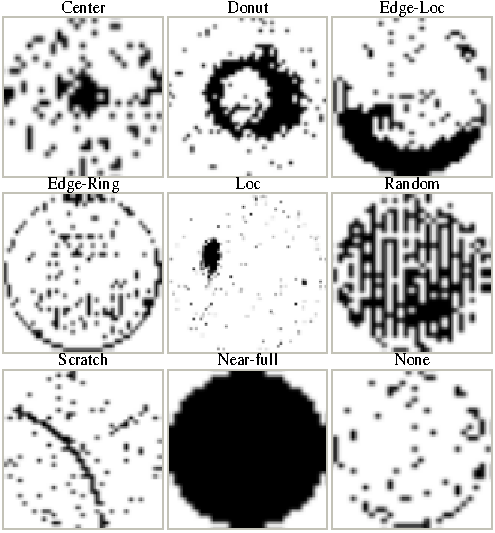
\includegraphics[width=0.85\columnwidth]{figures/examples_grid.pdf}
\caption{One test wafer map per class (dark: failed die; $64\times64$ CNN input).}
\label{fig:examples}
\end{figure}

\textbf{Handcrafted features (MFE).} The 59 features of~\cite{kang2021stacking}: 13 defect densities over fixed wafer
regions, 40 Radon-transform features (20 cubic-interpolated row means and 20 row standard deviations), and 6 geometric
properties of the most salient defect region (area, perimeter, major and minor axis length, eccentricity, solidity).
We use the authors' public feature-extraction code~\cite{dmkelllog_stacking} unchanged.

\textbf{Base classifiers.} \emph{MFE+FNN}: standardized features, two hidden layers of 128 tanh units, softmax output.
\emph{CNN}: the map is binarized (defective die $=1$), resized to $64\times64$, scaled to $[-1,1]$ and replicated to three
channels; the VGG16 convolutional stack~\cite{simonyan2015vgg}, initialized from ImageNet~\cite{russakovsky2015imagenet},
is followed by global average pooling and a softmax layer. Both are trained with Adam~\cite{kingma2015adam} (learning
rate $10^{-4}$, batch 32) and early stopping on validation loss (patience 20), as in~\cite{kang2021stacking}.

\textbf{Meta-classifiers.} Let $p_1, p_2 \in \mathbb{R}^9$ be the two class-probability vectors and $x=[p_1;p_2]$. The
proposed MLR meta-classifier is a ridge regression~\cite{hoerl1970ridge} of the one-hot label on $x$ (no intercept,
$\alpha=0.1$); the predicted class is the arg-max of the nine outputs, so each class receives its own weight for each base
classifier. Baselines: Stacking-FNN (one hidden layer of 10 units), Stacking-DT (a default scikit-learn decision
tree~\cite{pedregosa2011sklearn}), and MultiNN, a CNN whose pooled 512-dimensional features are concatenated with the 59
handcrafted features before the output layer~\cite{dmkelllog_multinn}.

\section{Experimental Protocol}
\label{sec:protocol}
\textbf{Splits.} The training set is split into $A$ (the first 130,356 maps, 80\%) and $B$ (the remaining 32,590). Base
classifiers are fitted on $A$; $B$ is split once, stratified, into halves $\Bfit$ and $\Bval$ (16,295 each). Base
classifiers early-stop on $\Bfit$, so their outputs on $B$ are not in-sample.

\textbf{Meta-training.} The original protocol fits the meta-classifier on the base classifiers' outputs for their own
training data (our ``$A$-mode''). We additionally fit it on $B$ (``$B$-mode''), where the base outputs behave like
test-time outputs. For model selection, stackers are scored by two-fold cross-fitting over $B$ ($\Bfit \leftrightarrow
\Bval$, predictions pooled over all of $B$); final $B$-mode stackers are fitted on 80\% of $B$ (the remaining 20\% serve
the FNN's early stopping).

\textbf{Selection discipline.} Every choice---hyperparameters, which extension to keep, the final pipeline---is made on
$B$. The test set is used only to report results. Reported variation is the standard deviation over runs, where runs
differ in the MFE+FNN seed (3 or 5 seeds; MLR is deterministic given its inputs) or in the stacker seed.

\textbf{Statistics.} Comparisons report the paired $t$-test across runs, as in~\cite{kang2021stacking}, and a paired
bootstrap~\cite{efron1993bootstrap} over wafers (2,000 resamples) of the macro-F1 difference, giving a 95\% interval
that reflects the limited number of rare-class wafers. \textbf{Inclusion rule:} an extension is kept if it improves the
$B$ score by more than the baseline's run-to-run standard deviation; extensions that fail are reported.

\textbf{Implementation.} TensorFlow~\cite{abadi2016tensorflow} (2.10 and 2.17; equivalence checked by re-predicting a
trained CNN within $1.2\times10^{-4}$), scikit-learn, scikit-image~\cite{vanderwalt2014skimage} and
XGBoost~\cite{chen2016xgboost}; single NVIDIA GPUs. A CNN trains in about two hours.

\section{Reproduction}
\label{sec:repro}
\subsection{Full training set}
Table~\ref{tab:repro} compares our reproduction with Table~7 of~\cite{kang2021stacking}. All six models land within or
above one reported standard deviation. The stack improves on both of its base classifiers, as claimed.

\begin{table}[t]
\centering
\caption{Reproduction at $N=162{,}946$: test macro- and micro-F1, ours vs.\ Kang and Kang~\cite{kang2021stacking} (Table~7,
10 replications). Stacking-DT and Stacking-MLR use the original protocol (meta-classifier fitted on in-sample outputs on $A$).}
\label{tab:repro}
\setlength{\tabcolsep}{3pt}
\resizebox{\columnwidth}{!}{%
\begin{tabular}{lccccl}
\toprule
& \multicolumn{2}{c}{macro-F1} & \multicolumn{2}{c}{micro-F1} & \\
\cmidrule(lr){2-3}\cmidrule(lr){4-5}
Model & ours & reported & ours & reported & runs \\
\midrule
\tabinput{tables/repro.tex}
\bottomrule
\end{tabular}}\\[2pt]
\footnotesize{$^\dagger$Hidden layer of 64 units, fitted on $B$; with the original $18\!\to\!10\!\to\!9$ architecture
on in-sample outputs the stack reached $0.8402 \pm 0.0393$ (class-weighted) or $0.6298 \pm 0.0904$ (unweighted).}
\end{table}

Three implementation details that the reference code handles differently were decisive. First, \emph{class weights hurt}:
the reference code trains the base classifiers with balanced class weights, but the paper mentions none; removing them
raised the MFE+FNN from 0.8147 to the reported level and also helped the CNN. Second, ImageNet initialization and
flip/rotation augmentation were needed for the CNN to reach the reported score (a from-scratch, class-weighted CNN
reached 0.8496). Third, mixed precision and larger batches cost about four macro-F1 points on this VGG network without
batch normalization, so all CNNs use 32-bit arithmetic and batch 32.

\subsection{The meta-training pitfall}
\label{sec:pitfall}
Fitting the meta-classifier on in-sample outputs, as in the reference implementation, produced a stack that never
predicted Near-full (F1 $=0$) although both base classifiers recognized it, with macro-F1 $0.6298 \pm 0.0904$. In-sample,
the base classifiers are almost always right and nearly certain, so the meta-classifier learns to follow the
arg-max and never learns when to distrust a base classifier; rare classes, seen a handful of times, are swamped. Class
weights mask the problem but leave it unstable across seeds ($0.8402 \pm 0.0393$). Fitting the meta-classifier on $B$,
where outputs are as uncertain as at test time, removes it (Table~\ref{tab:repro}). This is the classic recommendation of
stacking~\cite{wolpert1992stacked,ting1999issues}, but it is easy to miss, and the MLR stack of the paper---which is
linear and has few parameters---is far less affected than the FNN or tree meta-classifiers.

\subsection{Training-size sweep}
Table~\ref{tab:sweep} and Fig.~\ref{fig:sweep} repeat the sweep of~\cite{kang2021stacking} with the original protocol: for
each replicate, $N$ training maps are sampled at random, 80\% are used for fitting and 20\% for early stopping, and the
meta-classifiers are fitted on the fitting part. At $N=5{,}000$ and $50{,}000$ every model exceeds the reported value;
our CNN gains most ($+0.09$ at $N=5{,}000$), which we attribute to augmentation and the absence of class weights. At
$N=500$ our CNN matches the reported value, while the handcrafted-feature model and the stackers fall below it. Both sides show large variation
there: with 400 fitting maps, several rare classes are often absent altogether (Donut and Near-full in our first
replicate).

The sweep also shows the pitfall at work. With in-sample meta-training, Stacking-DT collapses at $N=500$ (0.268) because
the tree learns thresholds on near-one-hot probabilities that do not transfer to the test set. At $N=50{,}000$ the MLR
stack (0.876) falls \emph{below} our CNN (0.883): the CNN looks near-perfect in-sample, so the stack cannot learn when to
override it. The paper's claim that the stack beats both base classifiers therefore holds at $N=500$, 5,000 and 162,946
in our runs, but not at 50,000 under the original protocol.

\begin{table}[t]
\centering
\caption{Training-size sweep, test macro-F1 (ours / reported in~\cite{kang2021stacking}). Original protocol: in-sample
meta-training on the fitting part. Last row: full-data reproduction (Table~\ref{tab:repro}).}
\label{tab:sweep}
\setlength{\tabcolsep}{2.5pt}
\resizebox{\columnwidth}{!}{%
\begin{tabular}{rcccccc}
\toprule
$N$ & reps & MFE+FNN & CNN & Stack-DT & Stack-FNN & Stack-MLR \\
\midrule
\tabinput{tables/sweep.tex}
\bottomrule
\end{tabular}}
\end{table}

\begin{figure}[t]
\centering
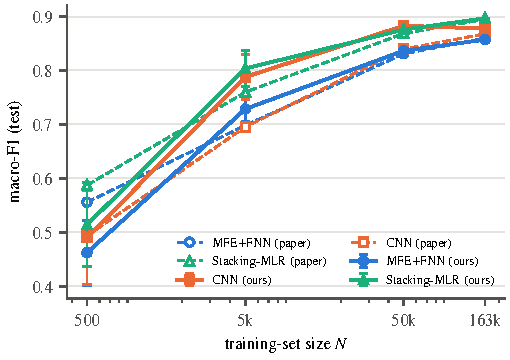
\includegraphics[width=\columnwidth]{figures/sweep.pdf}
\caption{Test macro-F1 against training-set size. Solid lines with filled markers: ours (mean $\pm$ std over replicates);
dashed lines with hollow markers: reported in~\cite{kang2021stacking}.}
\label{fig:sweep}
\end{figure}

\section{Extensions}
\label{sec:ext}
All extensions start from the corrected pipeline: MFE+FNN (5 seeds) and the CNN, both without class weights, with the
meta-classifier fitted on $B$. Table~\ref{tab:ext} lists every configuration; Table~\ref{tab:stats} gives the paired
comparisons.

\begin{table}[t]
\centering
\caption{Extensions. $B$: two-fold cross-fitted macro-F1 on $B$ (selection); test: macro-F1 on the 10,000 test maps.
CNN$\times$5: average of five CNN seeds, each with test-time augmentation. Rows without $\pm$: a single deterministic run.}
\label{tab:ext}
\setlength{\tabcolsep}{3pt}
\resizebox{\columnwidth}{!}{%
\begin{tabular}{lccc}
\toprule
Configuration & $B$ (MLR) & test (MLR) & test (FNN) \\
\midrule
\tabinput{tables/extensions.tex}
\bottomrule
\end{tabular}}
\end{table}

\begin{table}[t]
\centering
\caption{Paired comparisons (difference in macro-F1, $t$-test across runs, 95\% wafer-bootstrap interval).}
\label{tab:stats}
\setlength{\tabcolsep}{3pt}
\resizebox{\columnwidth}{!}{%
\begin{tabular}{llccc}
\toprule
Comparison & set & $\Delta$ & $p$ & 95\% CI \\
\midrule
\tabinput{tables/stats.tex}
\bottomrule
\end{tabular}}\\[2pt]
\footnotesize{$^\ddagger$Stack MFE-FNN + CNN$\times$5 + XGB vs.\ the CNN$\times$5 ensemble alone, on $\Bval$.}
\end{table}

\subsection{Test-time augmentation (TTA)}
Wafer defect patterns keep their class under rotation and reflection, so the CNN's prediction is averaged over the eight
symmetries of the square (four rotations, with and without a flip), without retraining. TTA passes the inclusion rule for
both meta-classifiers on $B$ (Table~\ref{tab:stats}) and raises the test macro-F1 of both stacks.

\subsection{A gradient-boosted third learner}
We added XGBoost~\cite{chen2016xgboost} on the same 59 features as a third base classifier, fitted on $A$ with the number
of trees chosen by early stopping on $\Bfit$. A 12-configuration grid (Appendix) was scored by the $B$ score of the
resulting stack; the selected model (depth 6, learning rate 0.05, balanced class weights) is also the best on its own
($\Bval$ macro-F1 0.8704 against 0.8525 for MFE+FNN). Two controls separate the possible explanations: replacing the
MFE+FNN with XGBoost (``is XGBoost simply better?'') and filling the third slot with a second MFE+FNN seed (``does any
third model help?''). The third learner passes the inclusion rule only for the FNN meta-classifier, and it never beats
the second-seed control significantly on $B$, so we find no evidence that a \emph{different kind} of learner helps.
Replacing the MFE+FNN with XGBoost gives the best $B$ score among single-CNN stacks.

\subsection{CNN seed ensembles}
Four further CNNs with the same recipe and different seeds reach the same validation loss (0.053--0.054) yet differ by
$\pm$\SeedStd{} in $\Bval$ macro-F1 (Appendix, Table~\ref{tab:seeds}): the rare classes swing between seeds. Averaging the
five TTA-CNNs~\cite{lakshminarayanan2017ensembles} gives the largest single improvement in this study ($+0.010$ on $B$
for the XGBoost stack, interval excluding zero).

\subsection{Final pipeline}
On $B$, the best configuration is the five-seed CNN ensemble with TTA plus XGBoost, combined by MLR. It reaches a test
macro-F1 of \FinalMacro{} and an accuracy of \FinalAcc\%, a gain of \GainOverRepro{} over our reproduced Stacking-MLR with a
bootstrap interval excluding zero. On the test set, the same stack with a single CNN scored slightly higher (0.9160); the
difference is well inside the bootstrap interval ($-0.0025$, $[-0.0143, +0.0091]$), and the ensemble was chosen on $B$.
Per-class F1 is given in the Appendix (Table~\ref{tab:perclass}).

\section{Selective Prediction}
\label{sec:reject}
In a fab, an uncertain wafer can be sent to an engineer. We convert the MLR scores to probabilities with a
temperature-scaled softmax (temperature $T=\CalT$ fitted by log-loss on the cross-fitted $B$ predictions) and accept a
wafer if its maximum probability exceeds a threshold. Thresholds are chosen on $B$ for target coverages and then applied to
the test set unchanged (Table~\ref{tab:reject}, Fig.~\ref{fig:reject}). Classifying \RejCov\% of wafers automatically
yields \RejAcc\% accuracy and a macro-F1 of \RejMacro{} on them; the deferred wafers are mostly Loc (44\% of that class),
Scratch (38\%), Edge-Loc (35\%) and Donut (25\%), while only 2\% of None wafers are deferred, which keeps the manual
workload small.

\begin{table}[t]
\centering
\caption{Reject option for the final pipeline on the test set. Thresholds chosen on $B$.}
\label{tab:reject}
\begin{tabular}{cccc}
\toprule
target & coverage & accuracy & macro-F1 \\
\midrule
\tabinput{tables/reject.tex}
\bottomrule
\end{tabular}
\end{table}

\begin{figure}[t]
\centering
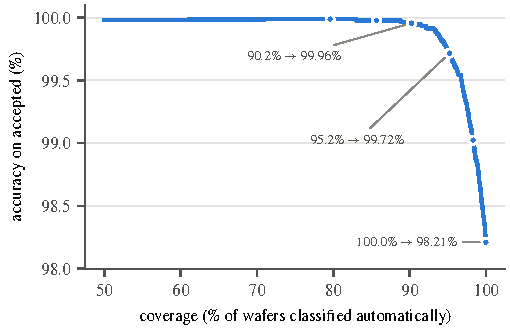
\includegraphics[width=\columnwidth]{figures/reject.pdf}
\caption{Risk--coverage curve of the final pipeline on the test set; markers: operating points with thresholds chosen on
$B$ (labels: coverage $\to$ accuracy).}
\label{fig:reject}
\end{figure}

\section{What the Stack Learns}
Fig.~\ref{fig:weights} shows the diagonal MLR weights---the weight each base classifier's vote for a class receives in
that class's score---for the two-learner stack with TTA. As in Fig.~5 of~\cite{kang2021stacking}, the handcrafted-feature
model carries Random and Near-full, which are defined by global density, while the CNN carries the spatial patterns such
as Edge-Ring and Scratch. In the three-learner stack, XGBoost takes over most of the Near-full weight from the MFE+FNN.
TreeSHAP~\cite{lundberg2017shap,lundberg2020treeshap} on the XGBoost model ranks geometric features (eccentricity,
solidity) highest for Scratch and the area of the defect region highest for Near-full; Grad-CAM~\cite{selvaraju2017gradcam}
maps of the CNN concentrate on the defect regions for correctly classified wafers (Appendix, Fig.~\ref{fig:gradcam}).

\begin{figure}[t]
\centering
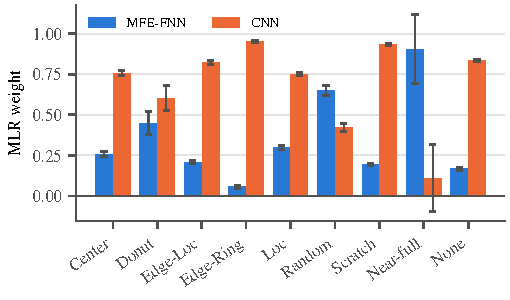
\includegraphics[width=\columnwidth]{figures/weights.pdf}
\caption{MLR weight of each base classifier's own-class vote (MFE-FNN + CNN with TTA; mean $\pm$ std over five MFE+FNN
seeds).}
\label{fig:weights}
\end{figure}

\section{Negative Results and Limitations}
\label{sec:neg}
\textbf{Negative results.} (i) Once the CNN is a five-seed ensemble, the original MFE+FNN no longer helps: the stack with
it scores below the CNN ensemble alone on $\Bval$ (Table~\ref{tab:stats}); handcrafted features still contribute a little
through XGBoost. (ii) A third learner of a different kind is not better than a second seed of the existing one.
(iii) Bagging XGBoost over five subsampled seeds improved it on its own ($\Bval$ 0.8785) but lowered every stack it entered
on $B$ by 0.0014--0.0018, so it was dropped. (iv) Temperature scaling did not improve calibration of the MLR stack: the
clipped and renormalized MLR outputs already have a test ECE of \EceRaw{}, against \EceT{} after scaling; it is still needed
to turn MLR scores into probabilities for the reject rule. (v) Class weights, mixed precision and a reduce-on-plateau
learning-rate schedule did not help. (vi) Under in-sample meta-training, Stacking-MLR does not beat the CNN at
$N=50{,}000$.

\textbf{Limitations.} We use one fixed train/test split, whereas~\cite{kang2021stacking} averages ten random splits; our
variation reflects seeds of the learners, and the wafer bootstrap covers sampling of the test set. Near-full has only nine
test wafers, so one wafer moves the macro-F1 by about 0.01. The test set was consulted twice---after the first round of
extensions and for the final pipeline---although every selection was made on $B$. The training-size sweep uses five
replicates at $N=50{,}000$ instead of ten, MultiNN is a single run, and the preliminary model-selection experiments
of~\cite{kang2021stacking} (their Tables~5--6) were not repeated.

\section{Conclusion}
The stacking ensemble of Kang and Kang reproduces: at full data our Stacking-MLR reaches \ReproMLR{} against the reported
0.8949, and the stack beats both base classifiers at three of four training sizes. Two practical lessons emerge. The
meta-classifier must be trained on outputs for data the base classifiers did not fit, or it learns to trust over-confident
in-sample predictions. And the value of the handcrafted-feature branch depends on how strong the CNN is: against a single
CNN it helps, against a five-seed ensemble with test-time augmentation it no longer does. Our best pipeline reaches a
macro-F1 of \FinalMacro{} and, with a reject option, classifies \RejCov\% of wafers at \RejAcc\% accuracy.

\section*{Code Availability}
Code, logs and result files are available at
\url{https://github.com/Kartikeya2046/ML_wafer_detecting_using_stack_ensemble}. Every table in this paper is generated from
the saved outputs by a script in that repository.

\bibliographystyle{IEEEtran}
\bibliography{refs}

\clearpage
\section*{Appendix}

\begin{table}[h]
\centering
\caption{Per-class test F1: reported Stacking-MLR~\cite{kang2021stacking} (Table~8), our reproduction, and our final pipeline.}
\label{tab:perclass}
\setlength{\tabcolsep}{4pt}
\begin{tabular}{lrccc}
\toprule
Class & $n$ & reported & reproduction & final \\
\midrule
\tabinput{tables/perclass.tex}
\bottomrule
\end{tabular}
\end{table}

\begin{table}[h]
\centering
\caption{CNN seeds (same recipe). Macro-F1 on $\Bval$ and test.}
\label{tab:seeds}
\begin{tabular}{lccc}
\toprule
seed & $\Bval$ & $\Bval$ (TTA) & test (TTA) \\
\midrule
\tabinput{tables/seeds.tex}
\bottomrule
\end{tabular}
\end{table}

\begin{table}[h]
\centering
\caption{XGBoost grid, ordered by the $B$ score of the three-learner MLR stack (selection criterion).}
\label{tab:xgb}
\setlength{\tabcolsep}{3pt}
\resizebox{\columnwidth}{!}{%
\begin{tabular}{cccccc}
\toprule
depth & lr & class weights & trees & $\Bval$ alone & stack ($B$) \\
\midrule
\tabinput{tables/xgbgrid.tex}
\bottomrule
\end{tabular}}
\end{table}

\begin{figure*}[t]
\centering
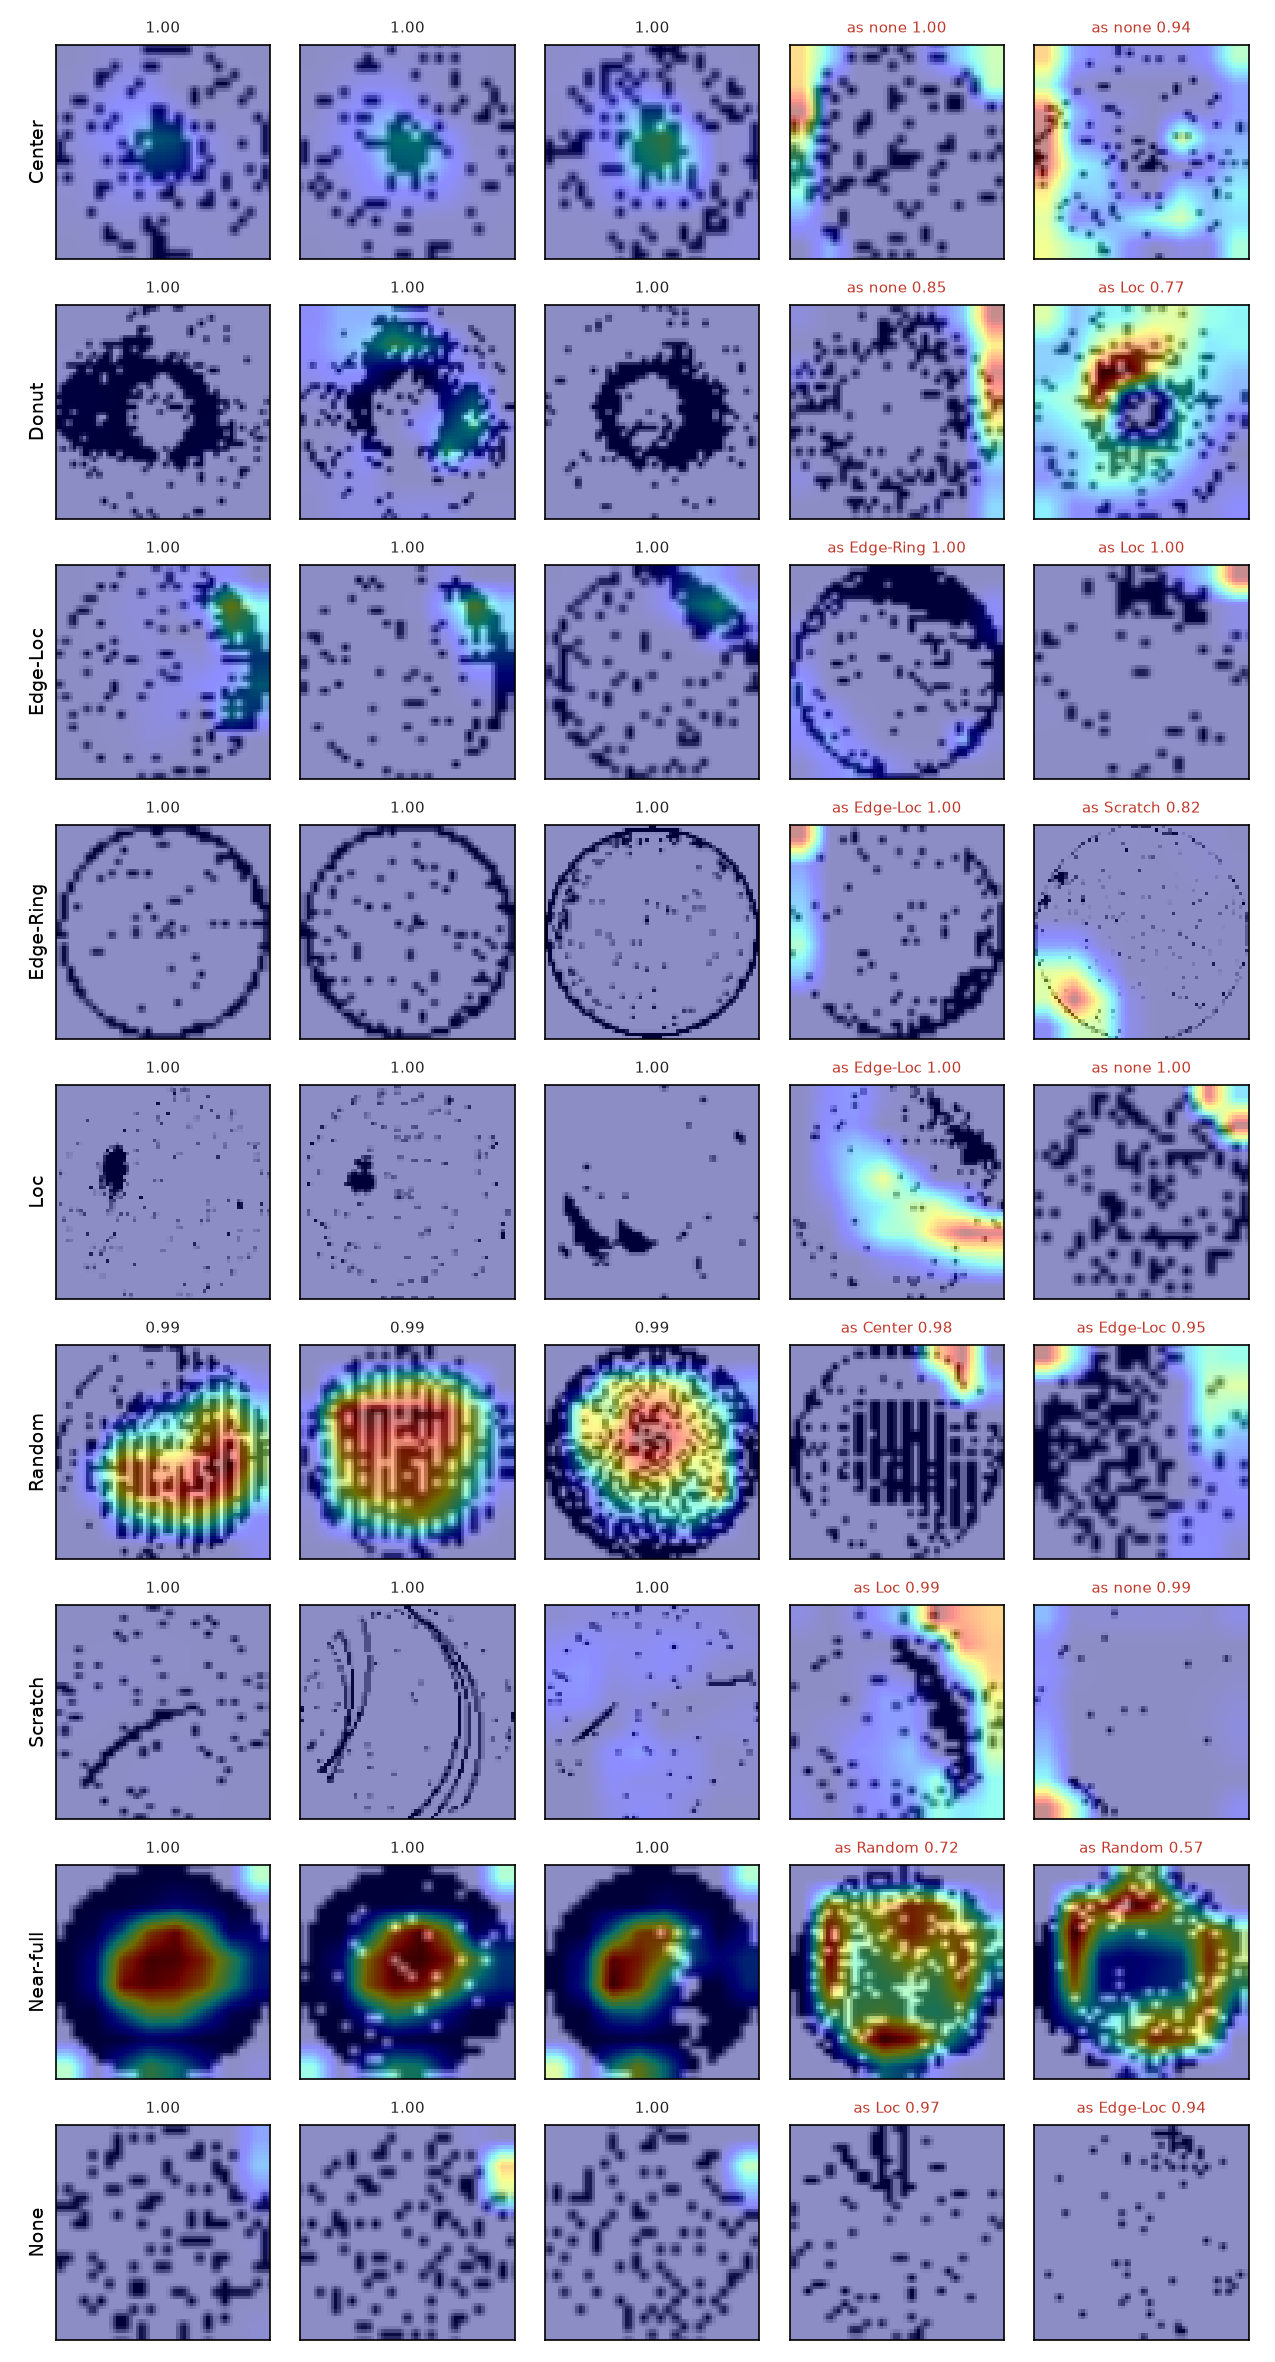
\includegraphics[width=0.62\textwidth]{figures/gradcam.png}
\caption{Grad-CAM~\cite{selvaraju2017gradcam} on test wafers (layer block4\_conv3, $8\times8$): three correctly classified
maps per class (left) and up to two misclassified maps (right, red titles). Confident correct maps of some classes are
nearly blank because the softmax is saturated, a known limitation of gradient-based maps.}
\label{fig:gradcam}
\end{figure*}

\end{document}
